% Appendix A

\chapter{Figures} % Main appendix title

\label{Figures} % For referencing this appendix elsewhere, use \ref{AppendixA}

%%%%% Introduction %%%%%

%%%%% Matériel et méthodes %%%%%

\begin{table}
\resizebox{19cm}{!}{
\begin{tabular}{| p{4cm} || l | l | p{5cm} | l | l |}
\hline
Système d'explotation & Processeur & Mémoire vive & Carte graphique\\ \hline
Ubuntu 16.04.4 & Intel Xeon E5-1607 (3,1GHz) &  
40 GB & NVIDIA GeForce GTX1060\\ \hline
\end{tabular}
}
\caption[Tableau]{Matériel utilisé pour réaliser les modélisations}
\label{tab:materiel}
\end{table}

\begin{figure}[th]
\centering
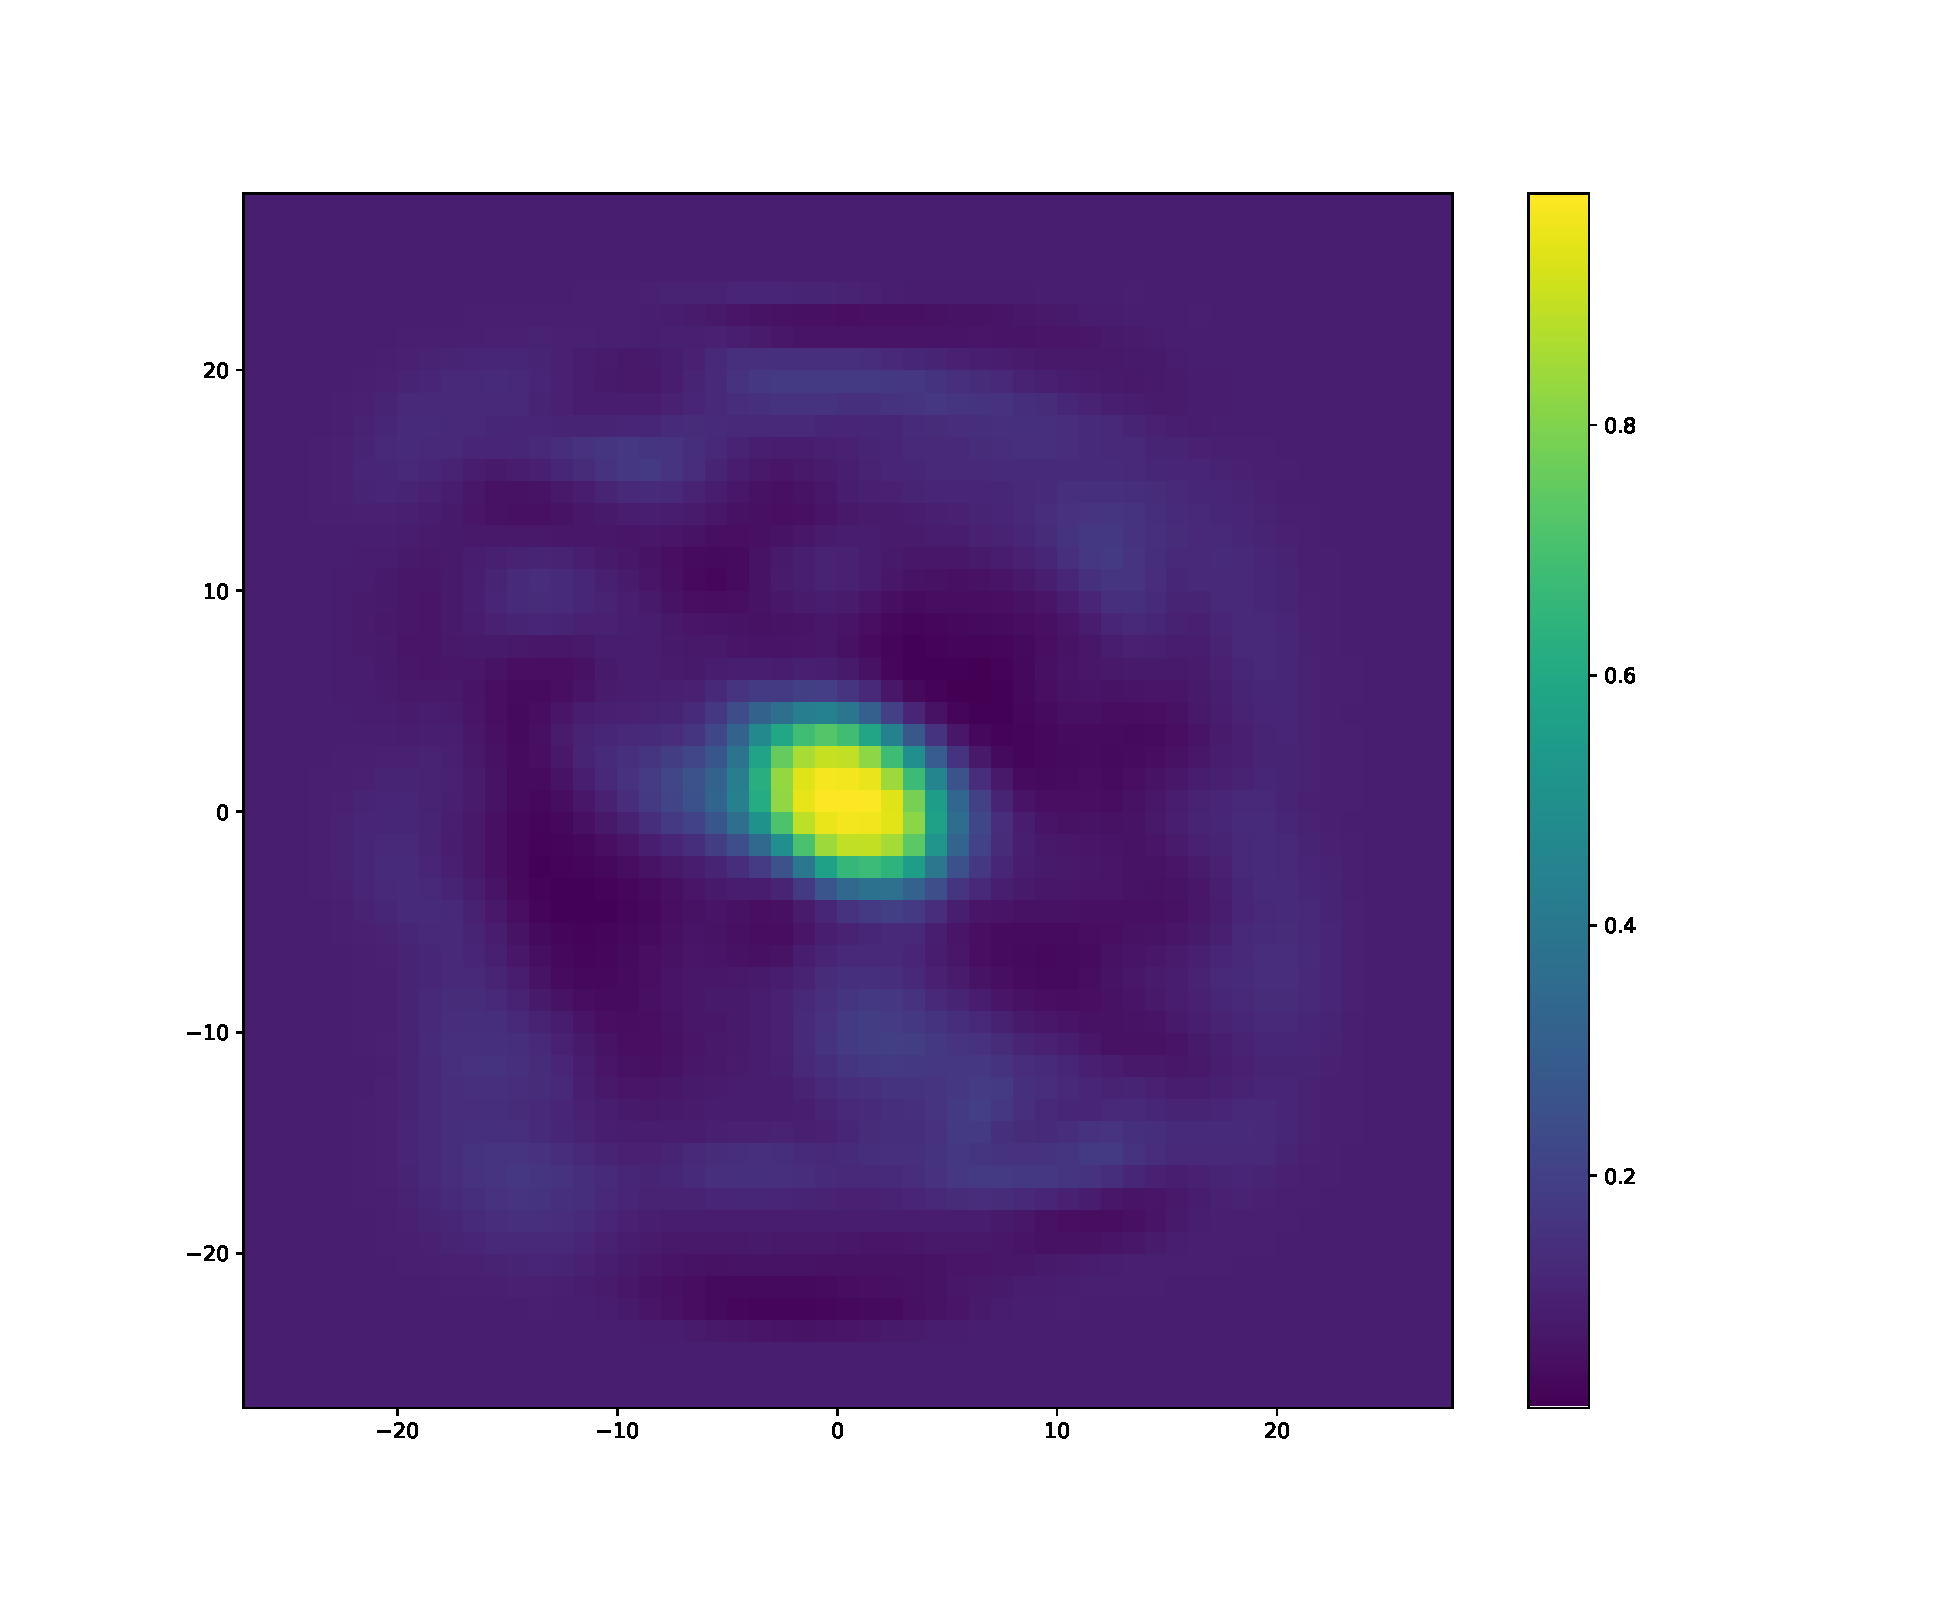
\includegraphics[scale=0.4]{Figures/accuracy}
\decoRule
\caption[Figure]{Reconstruction en carte de chaleur de la matrice de certitude}
\label{fig:accuracy}
\end{figure}

\begin{figure}[th]
\centering
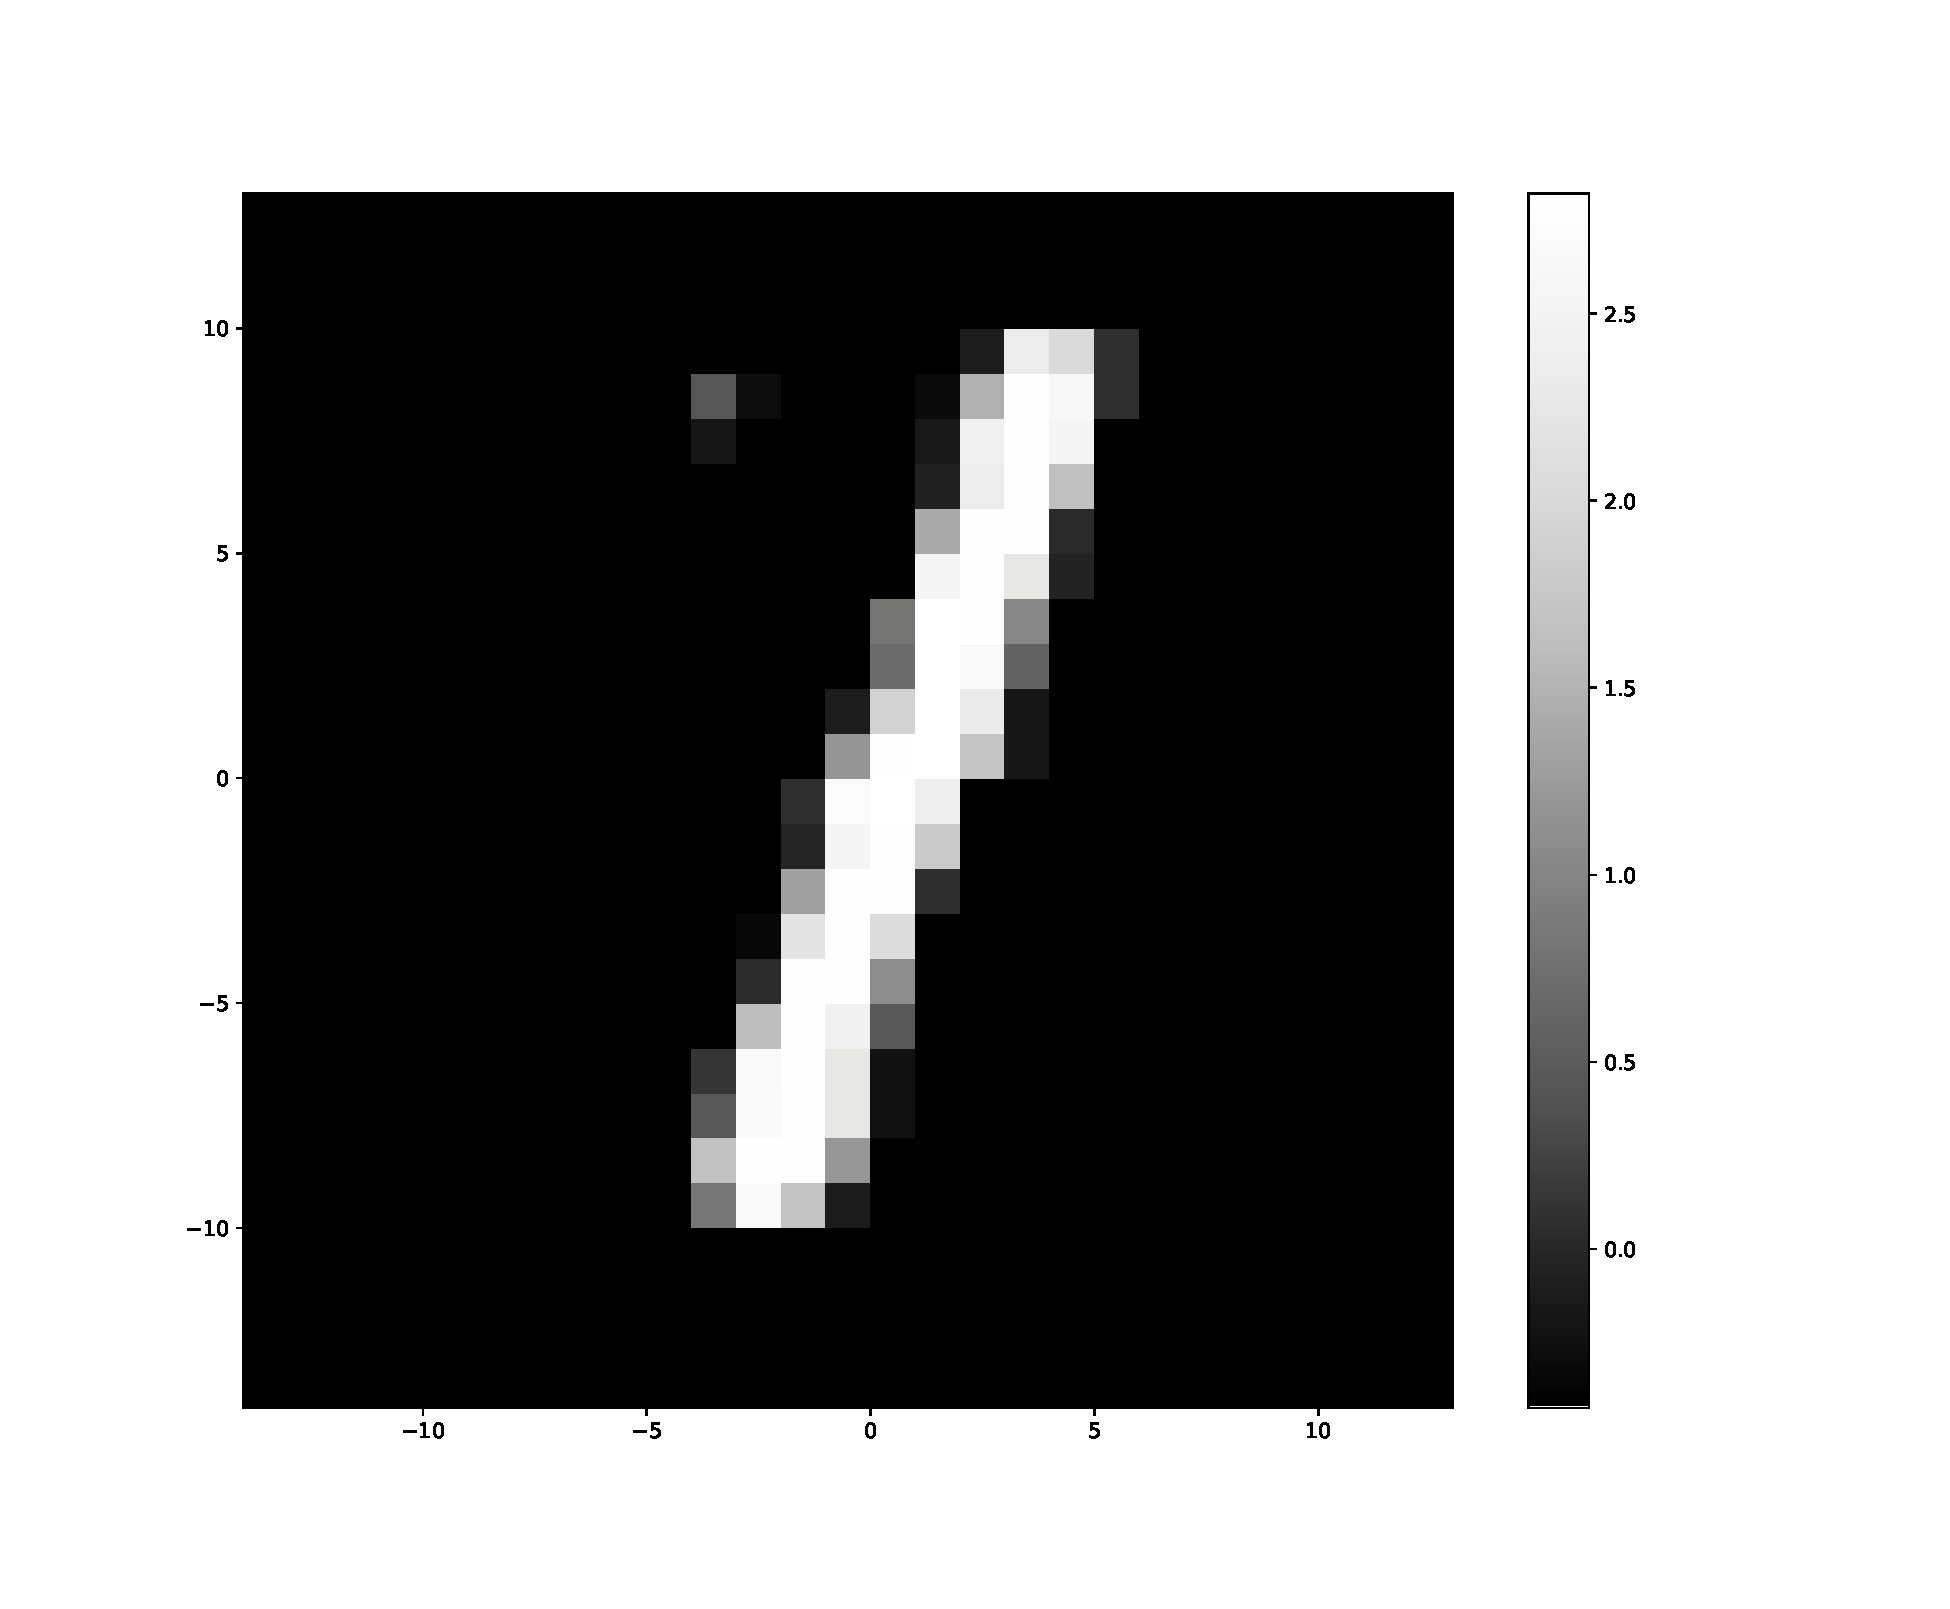
\includegraphics[scale=0.3]{Figures/MNIST_28}
\decoRule %puts an aesthetic horizontal line below the image
\caption[Figure]{Reconstruction en carte de chaleur d'une image provenant de la base de données MNIST}
\label{fig:MNIST_28}
\end{figure}

\begin{figure}[th]
\centering
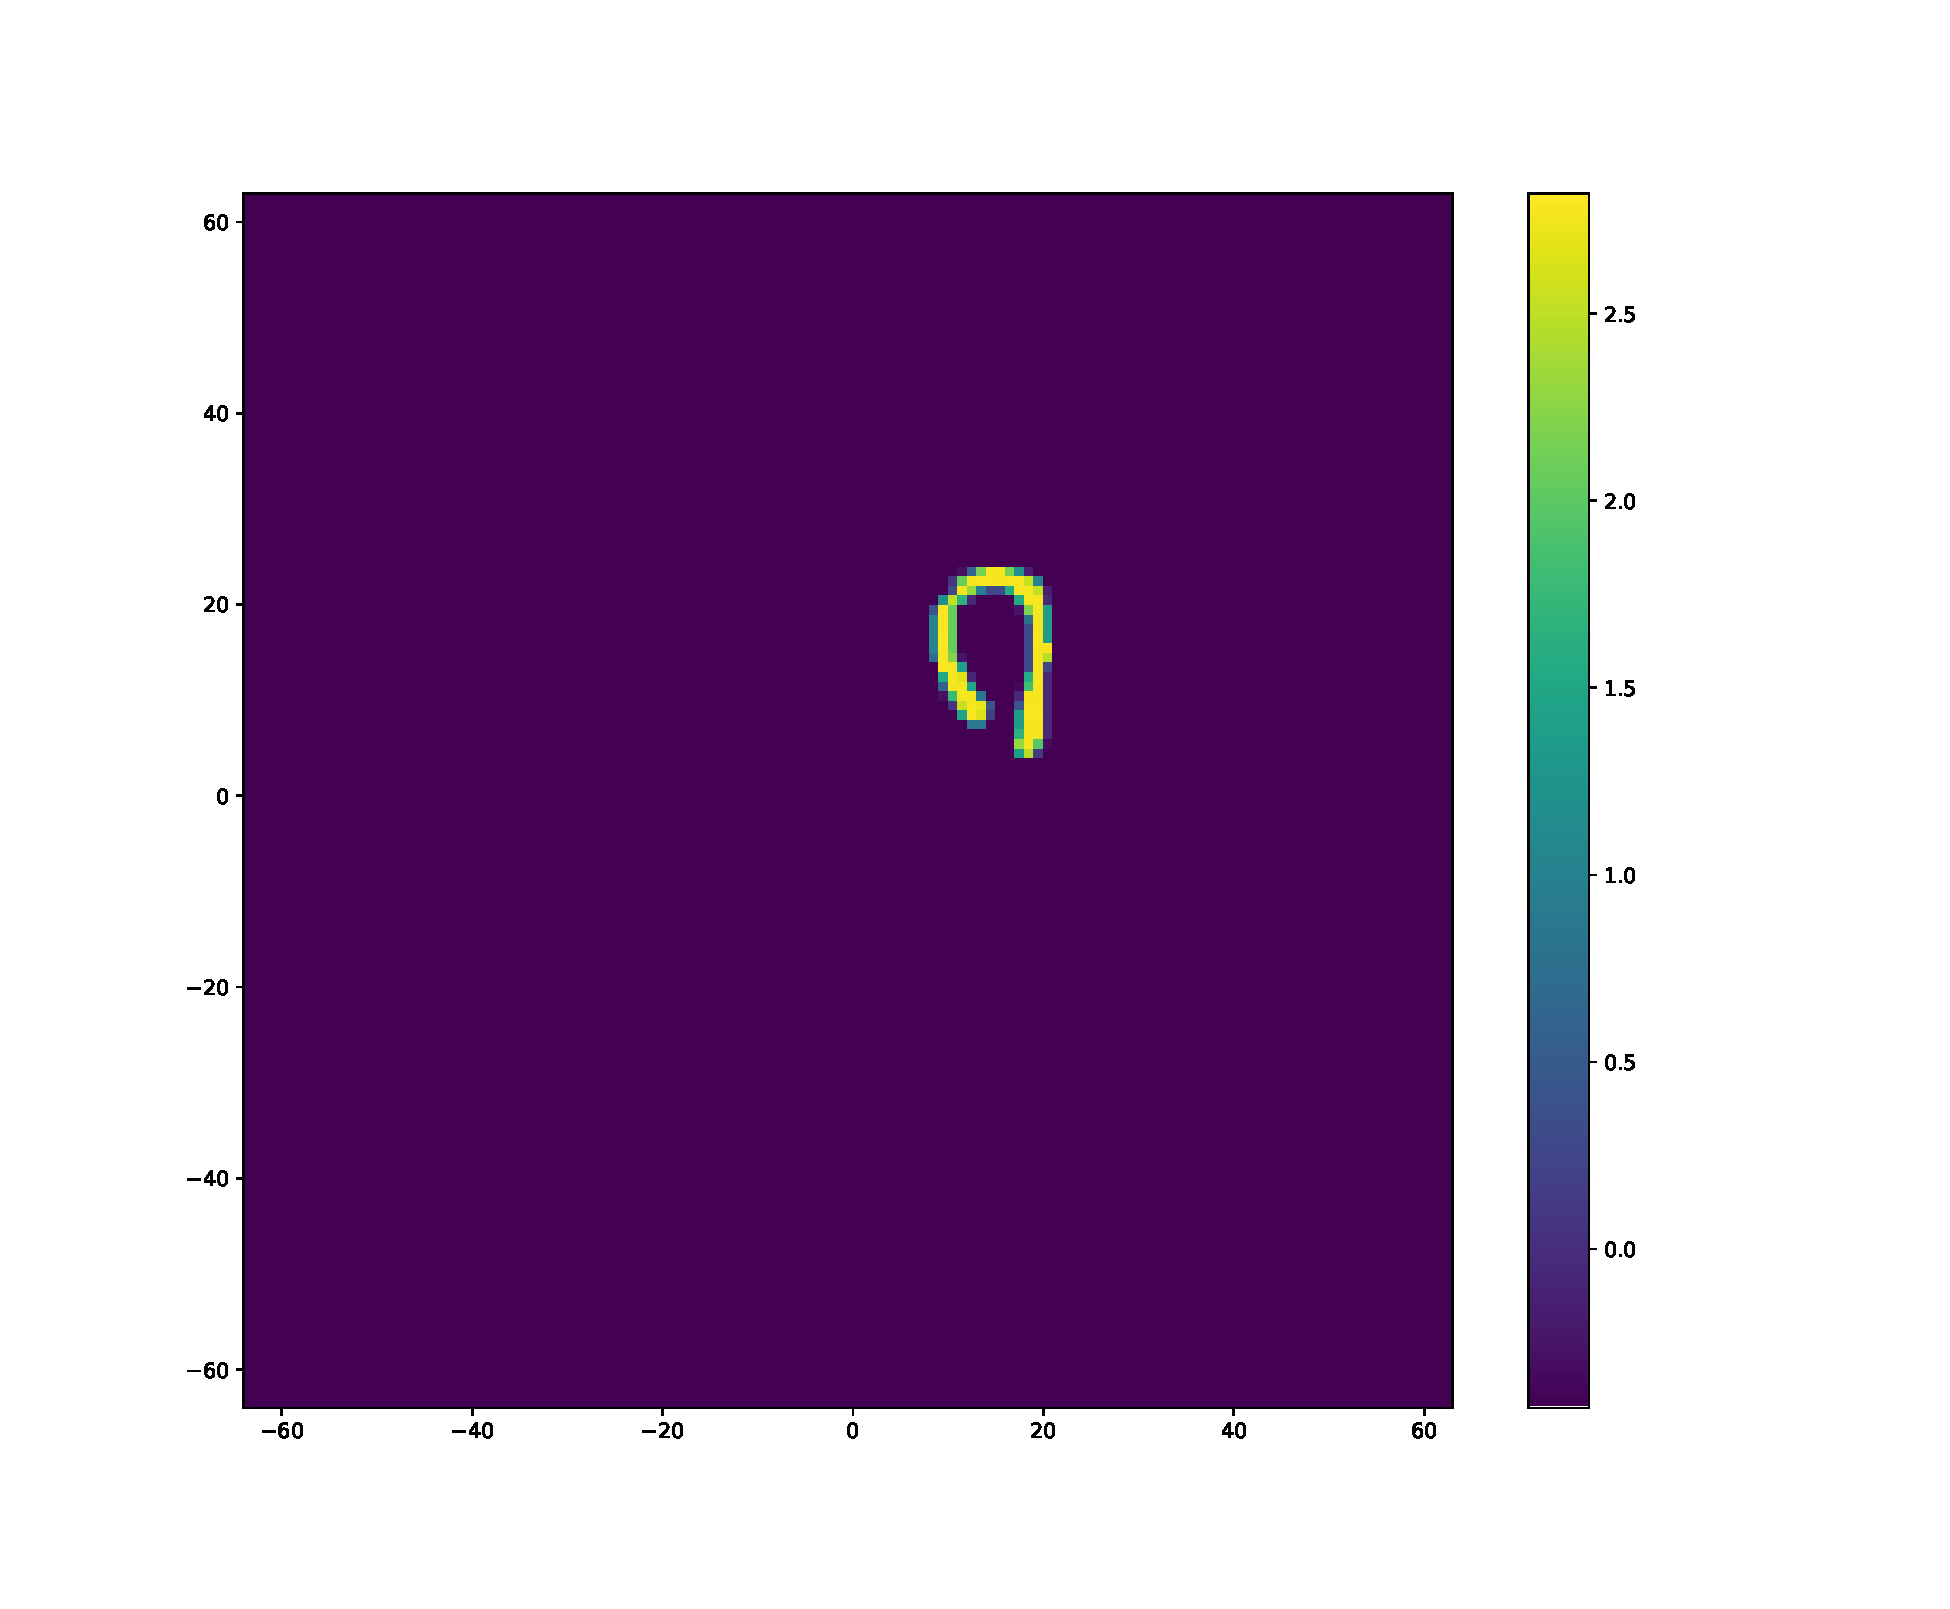
\includegraphics[scale=0.3]{Figures/MNIST_128}
\decoRule
\caption[Figure]{Reconstruction en carte de chaleur d'une image provenant de la base de données MNIST, après transformation pour la placer dans une image de dimension 128*128 pixels}
\label{fig:MNIST_128}
\end{figure}

\begin{figure}[th]
\centering
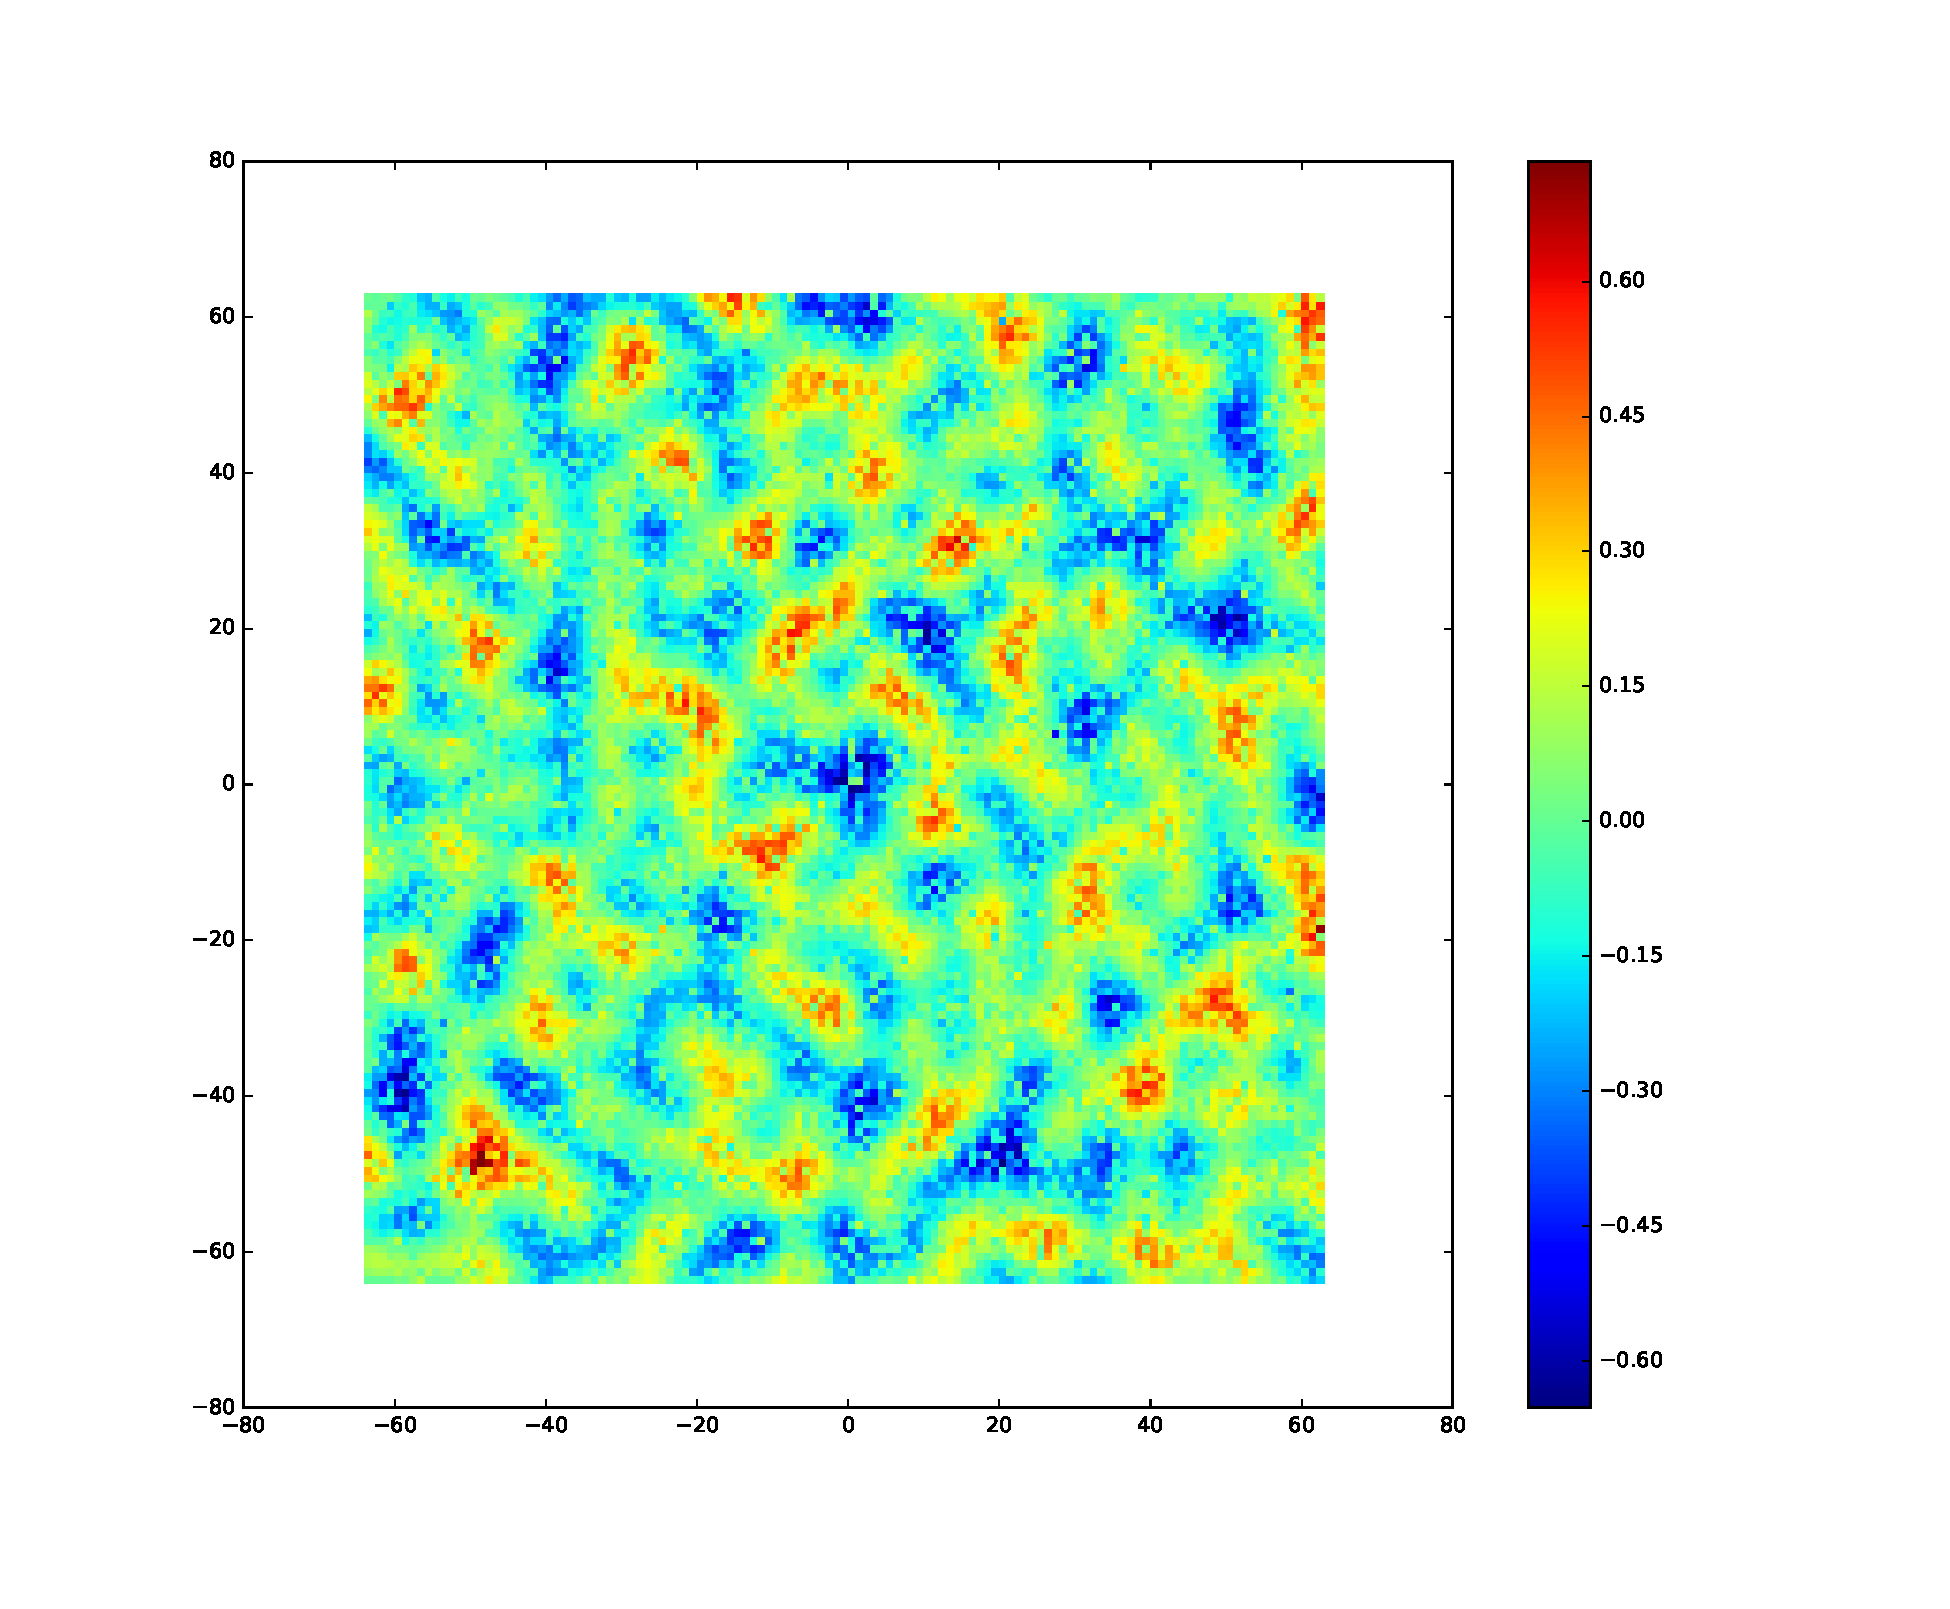
\includegraphics[scale=0.4]{Figures/perlin_noise}
\decoRule
\caption[Figure]{Reconstruction en carte de chaleur d'un bruit Perlin généré automatiquement et aléatoirement \autocite{Perlin1985}}
\label{fig:perlin_noise}
\end{figure}

\begin{figure}[th]
\centering
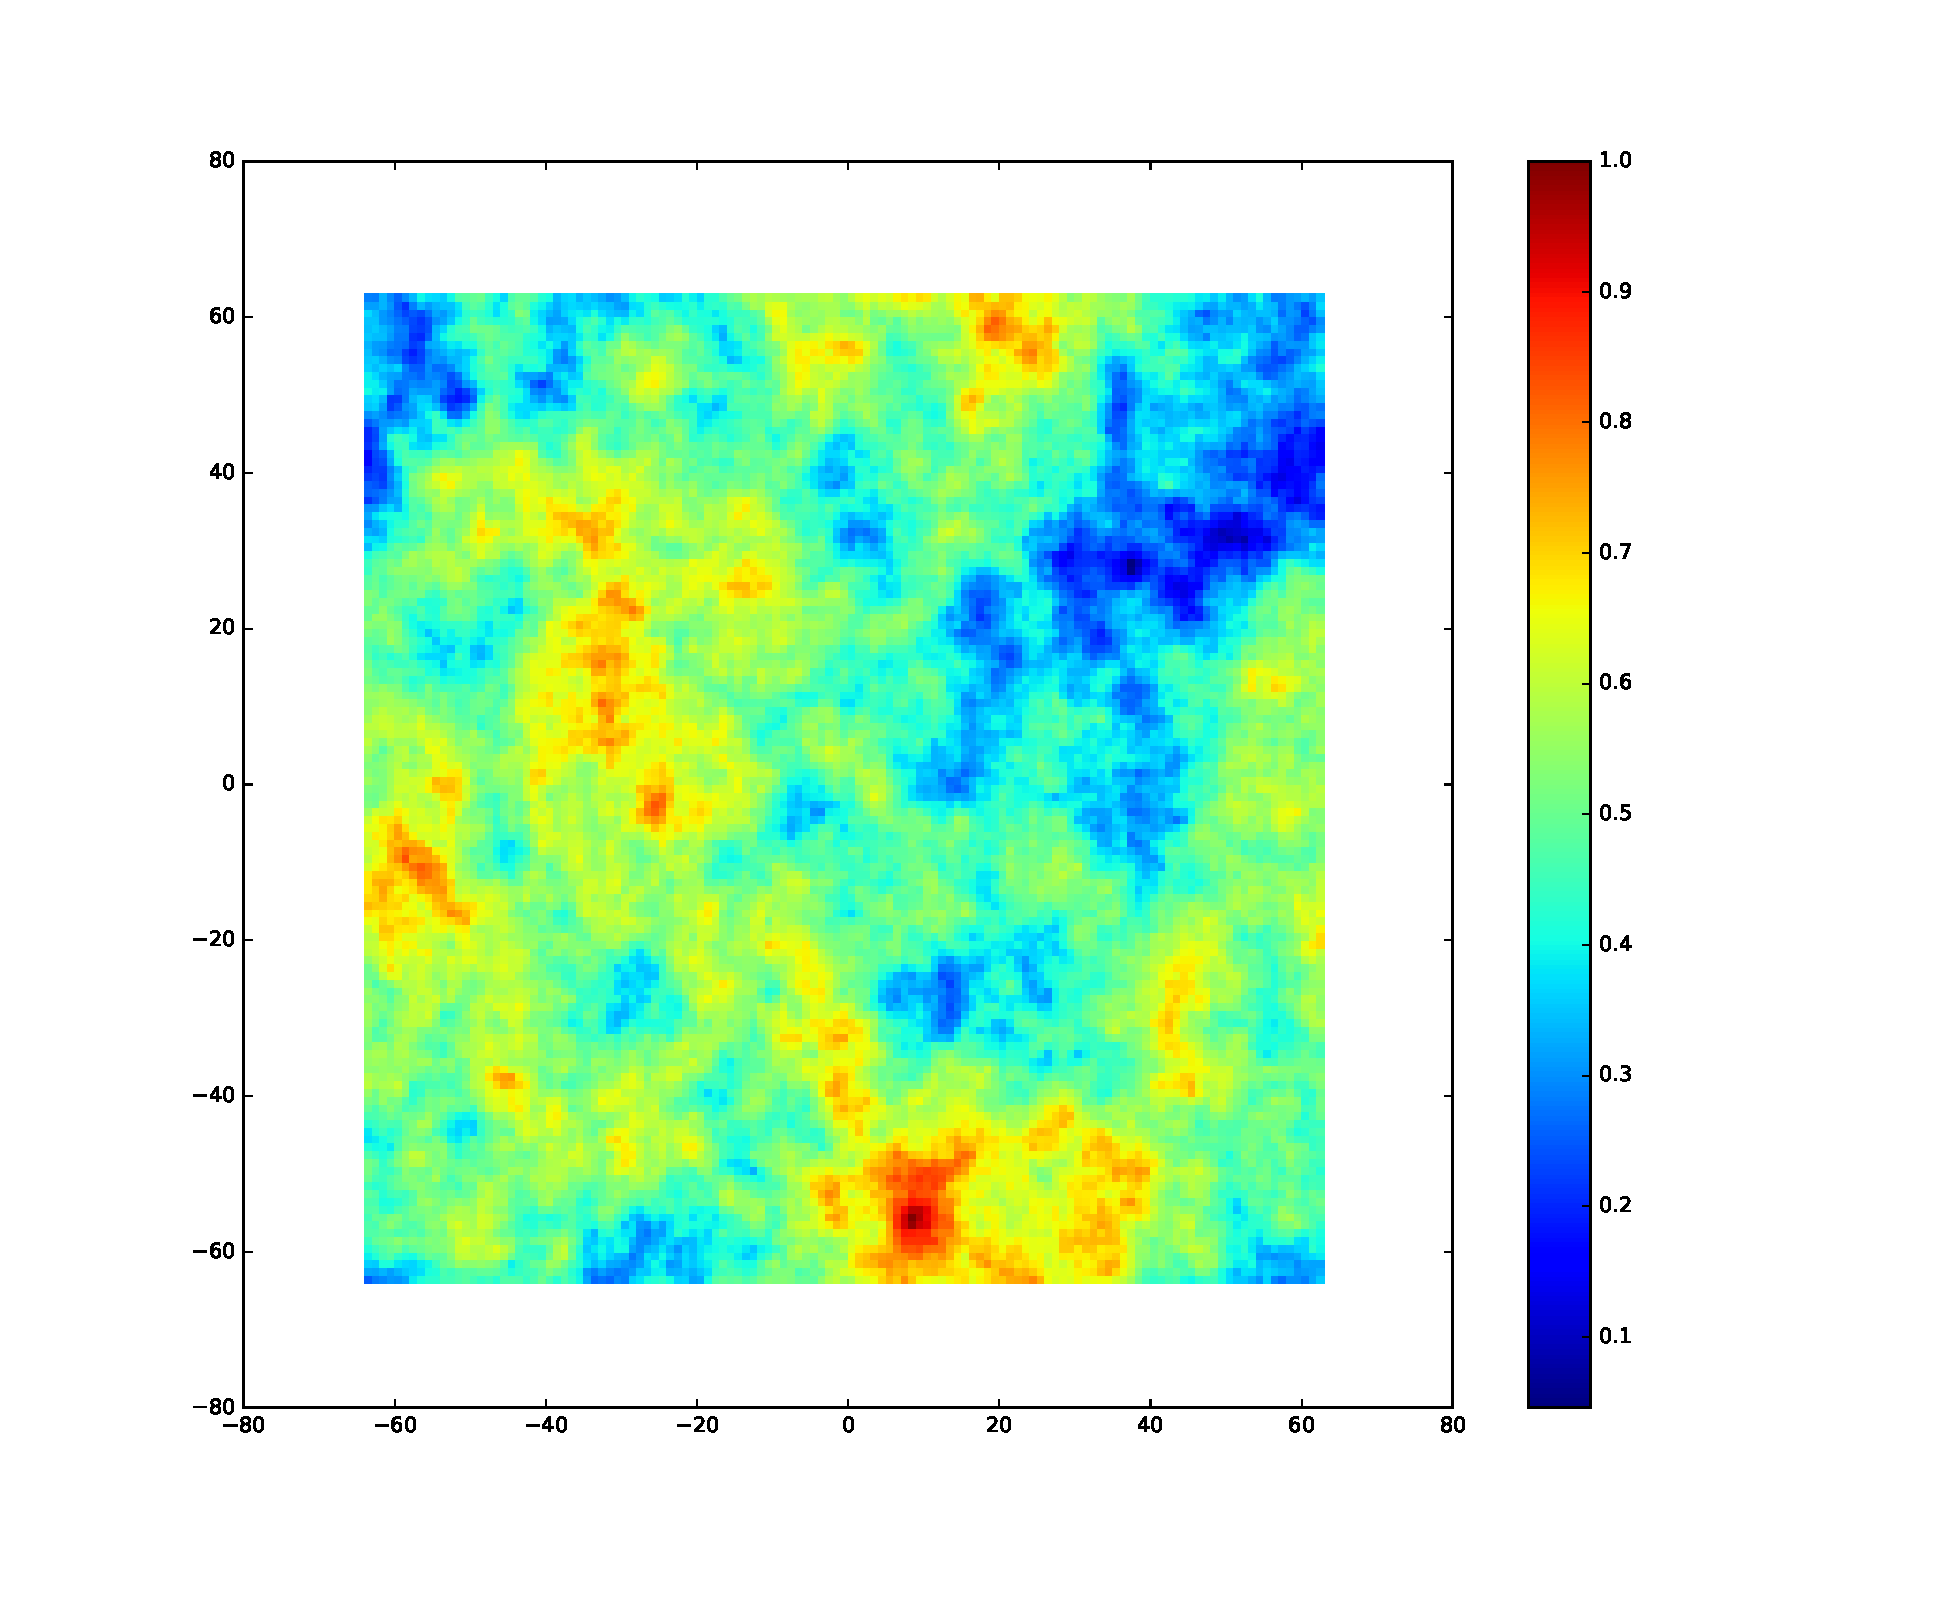
\includegraphics[scale=0.4]{Figures/motioncloud_noise}
\decoRule
\caption[Figure]{Reconstruction en carte de chaleur d'un bruit MotionCloud généré automatiquement et aléatoirement \autocite{Leon2012}}
\label{fig:motioncloud_noise}
\end{figure}

\begin{figure}[th]
\centering
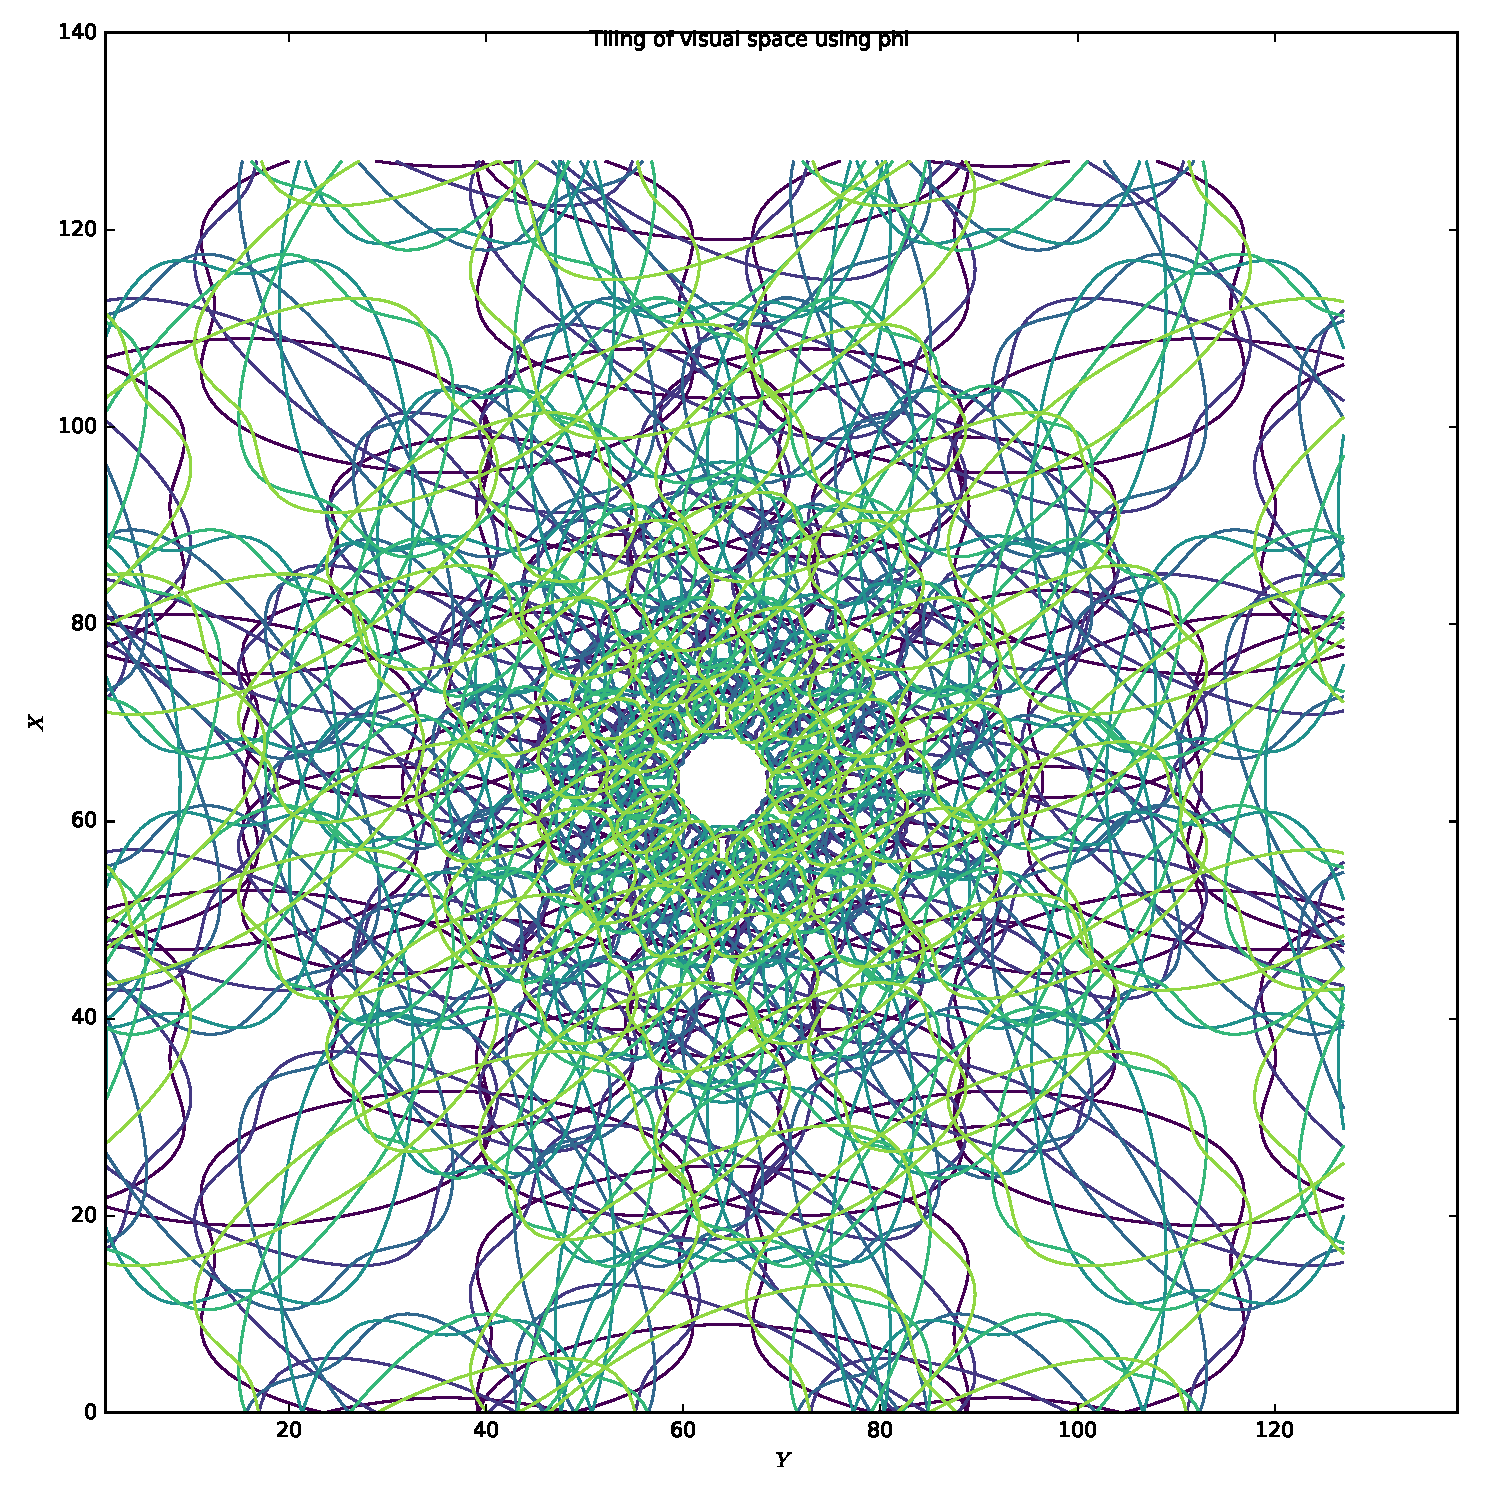
\includegraphics[scale=0.4]{Figures/logpol_filter}
\decoRule
\caption[Figure]{Schéma représentant le filtre LogPolaire pour les paramètres (Theta=6, Orient=12, Scale=5, Phase=2, Rho=1.61803). Chaque ovoïde représente un champs récepteur, modélisé par un filtre Gabor \autocite{Freeman2011}}
\label{fig:logpol_filter}
\end{figure}

\begin{figure}[th]
\centering
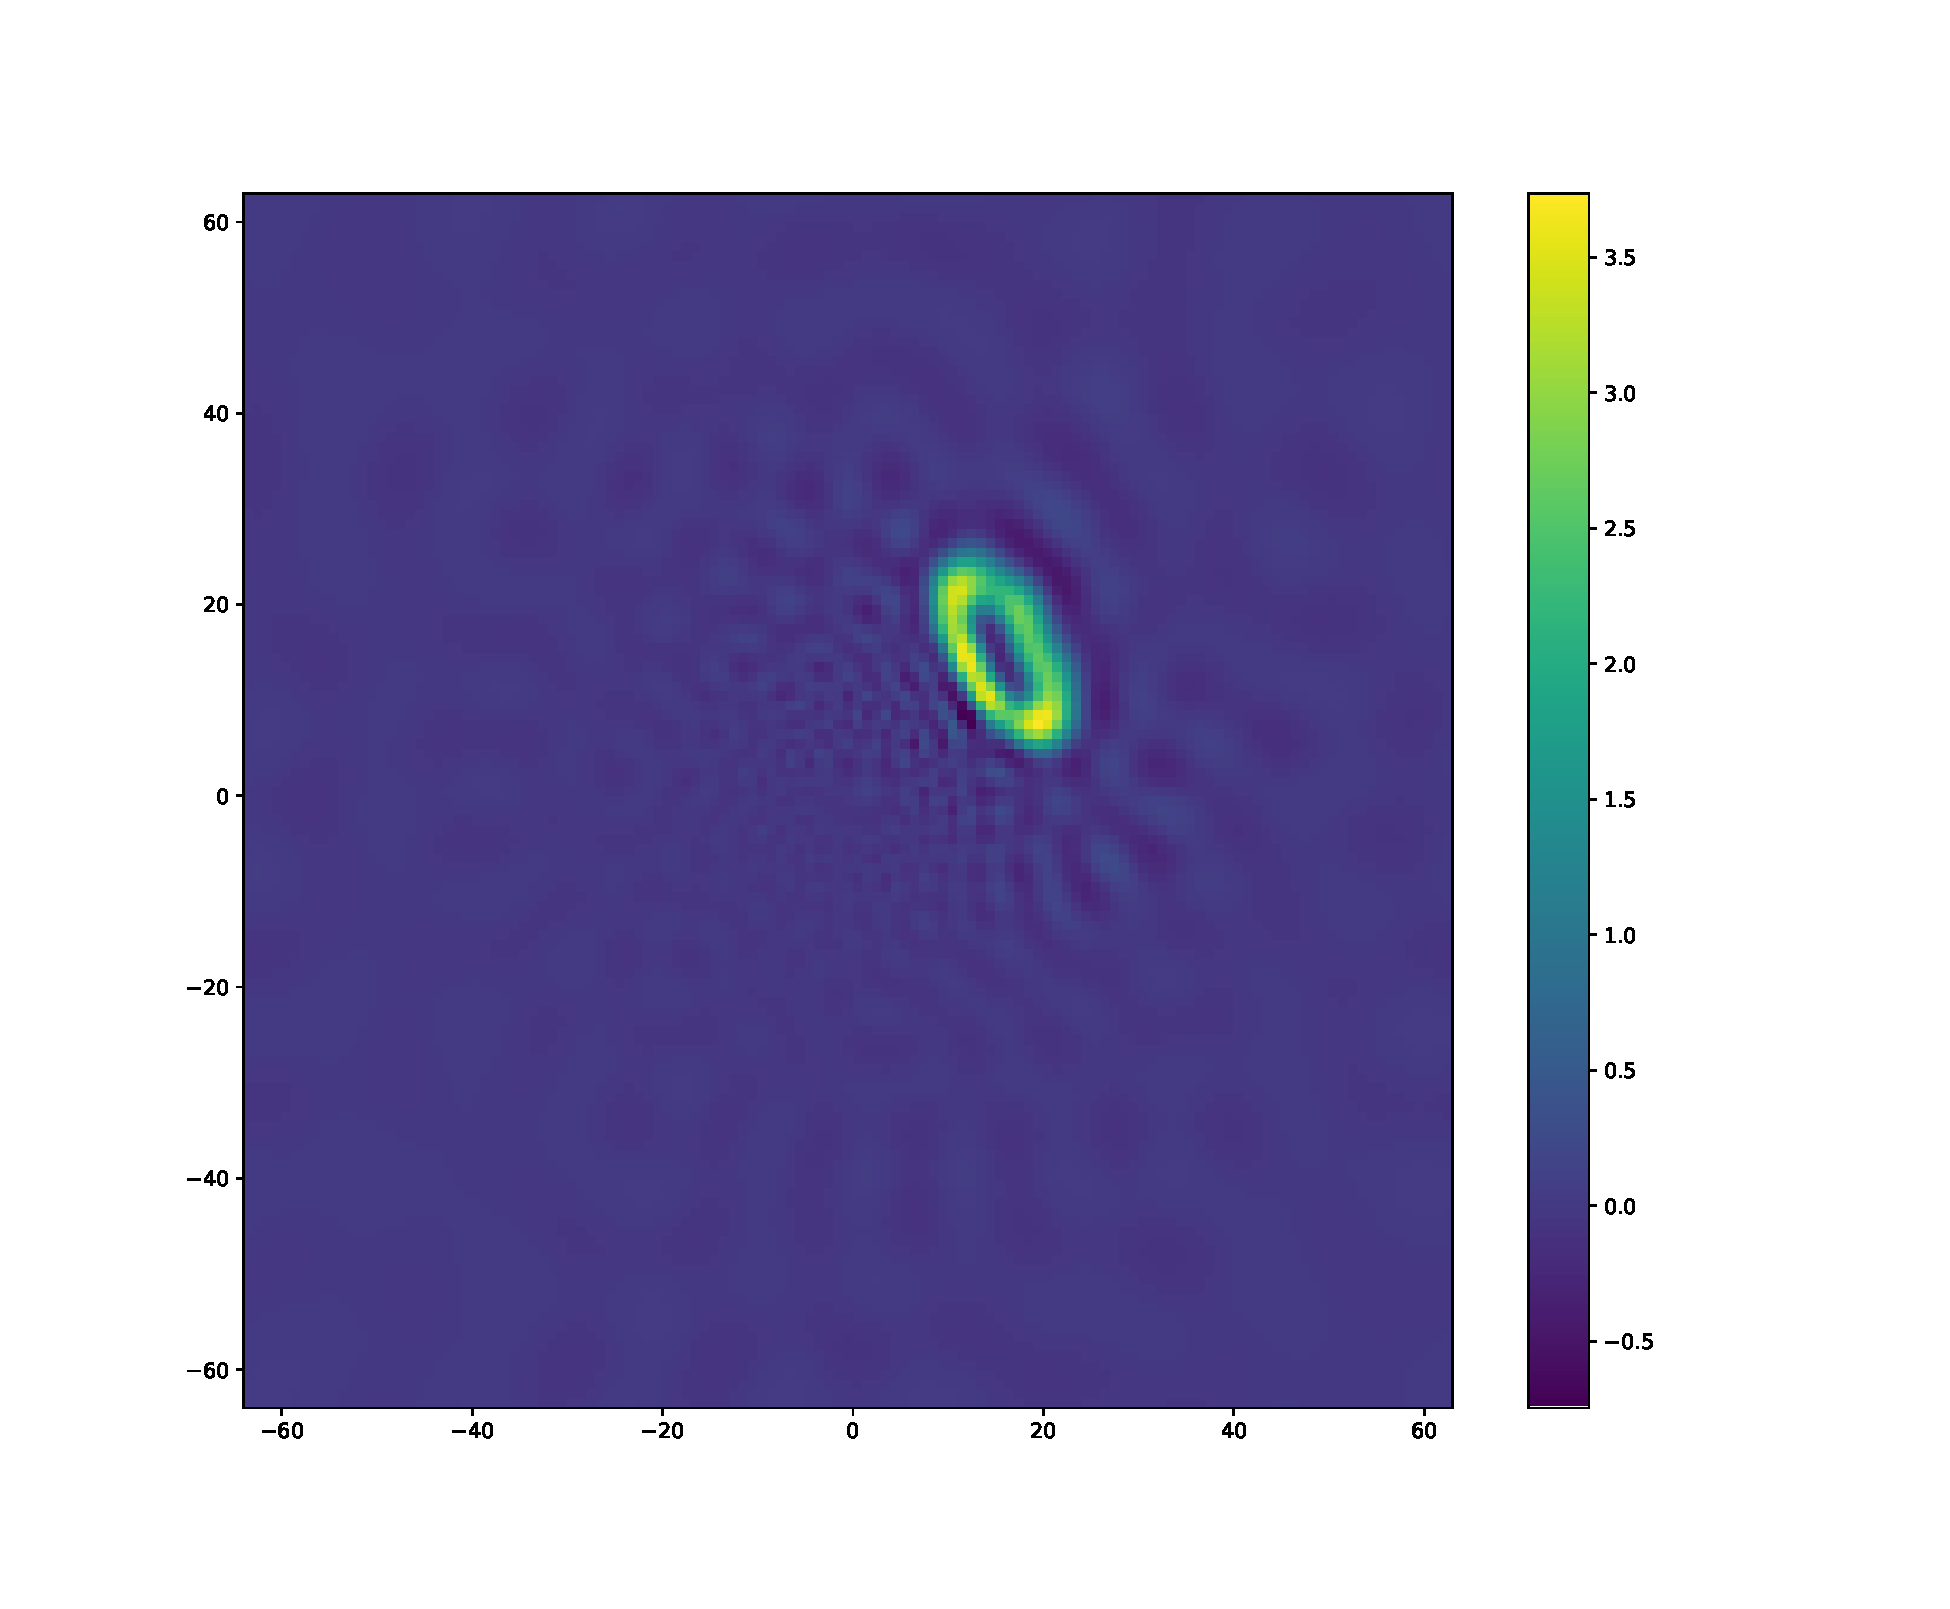
\includegraphics[scale=0.4]{Figures/mnist_128_LP_nonoise}
\decoRule
\caption[Figure]{Reconstruction en carte de chaleur d'un stimulus non-bruité après passage dans le filtre rétinien LogPolaire}
\label{fig:mnist_128_LP_nonoise}
\end{figure}

\begin{figure}[th]
\centering
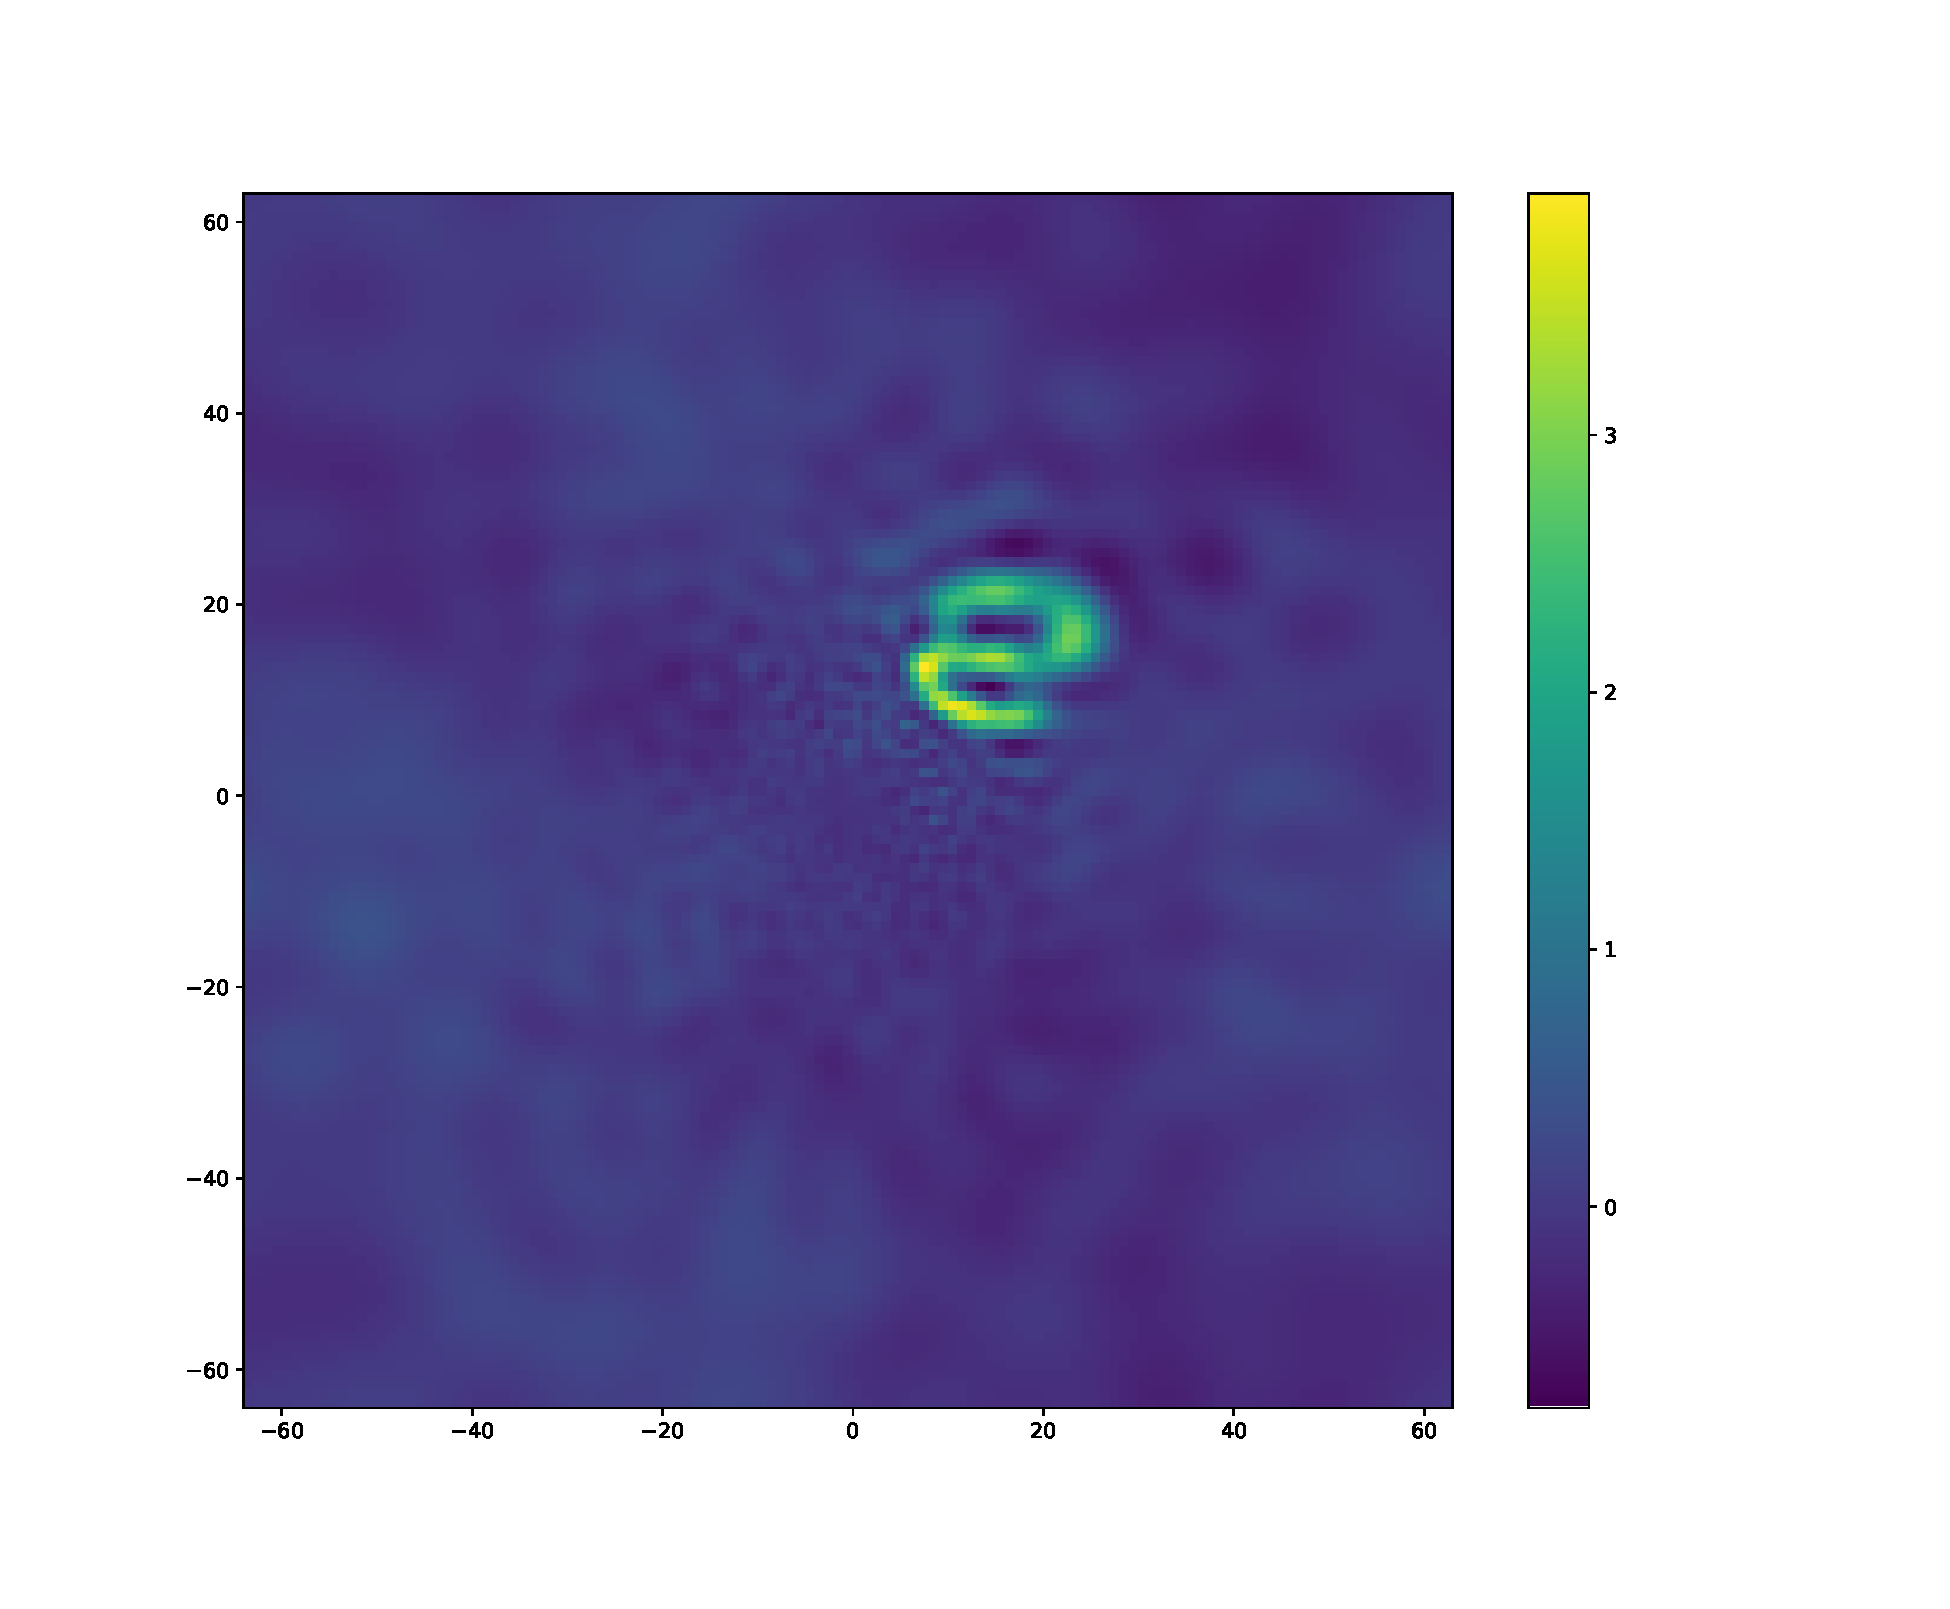
\includegraphics[scale=0.4]{Figures/mnist_128_LP_MotionCloud}
\decoRule
\caption[Figure]{Reconstruction en carte de chaleur d'un stimulus bruité par la méthode MotionCloud après passage dans le filtre rétinien LogPolaire}
\label{fig:mnist_128_LP_MotionCloud}
\end{figure}

\begin{figure}[th]
\centering
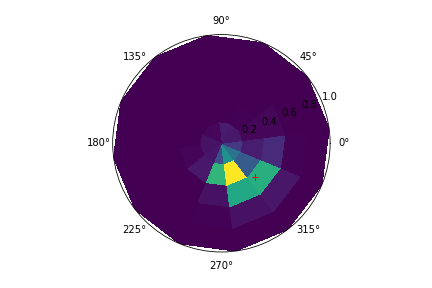
\includegraphics[scale=0.4]{Figures/mnist_log_nonoise}
\decoRule
\caption[Figure]{Reconstruction en graphique logarithmique d'un stimulus non-bruité après passage dans le filtre rétinien LogPolaire}
\label{fig:mnist_log_nonoise}
\end{figure}

\begin{figure}[th]
\centering
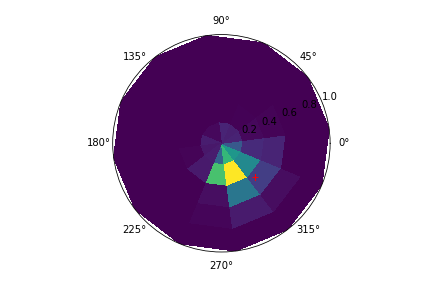
\includegraphics[scale=0.4]{Figures/mnist_log_motioncloud}
\decoRule
\caption[Figure]{Reconstruction en graphique logarithmique d'un stimulus bruité par la méthode MotionCloud après passage dans le filtre rétinien LogPolaire}
\label{fig:mnist_log_motioncloud}
\end{figure}

\begin{figure}[th]
\centering
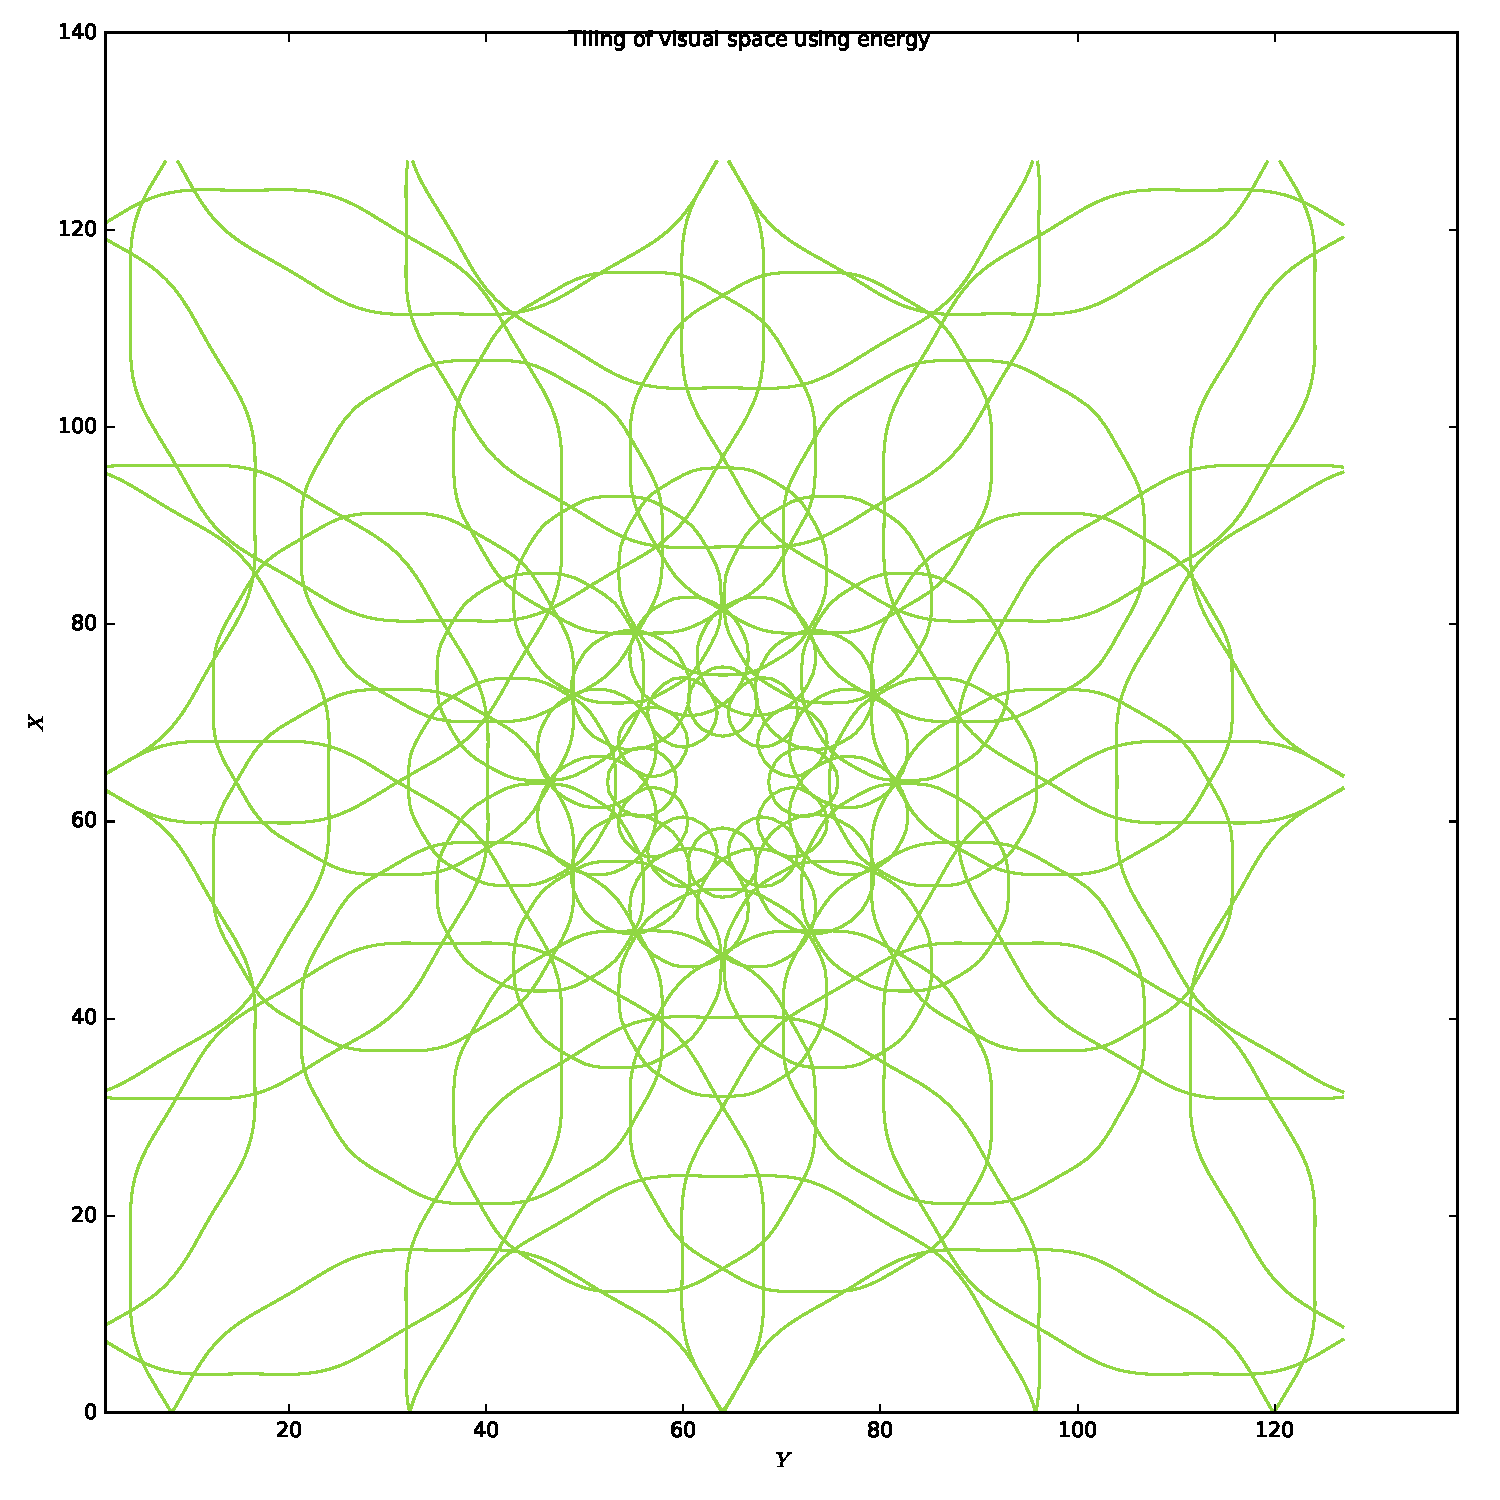
\includegraphics[scale=0.4]{Figures/logpol_energy_filter}
\decoRule
\caption[Figure]{Schéma représentant le filtre LogPolaire énergétique pour les paramètres (Orient=12, Scale=5, Rho=1.61803). Chaque cercle représente un champs récepteur}
\label{fig:energy_filter}
\end{figure}

\begin{figure}[th]
\centering
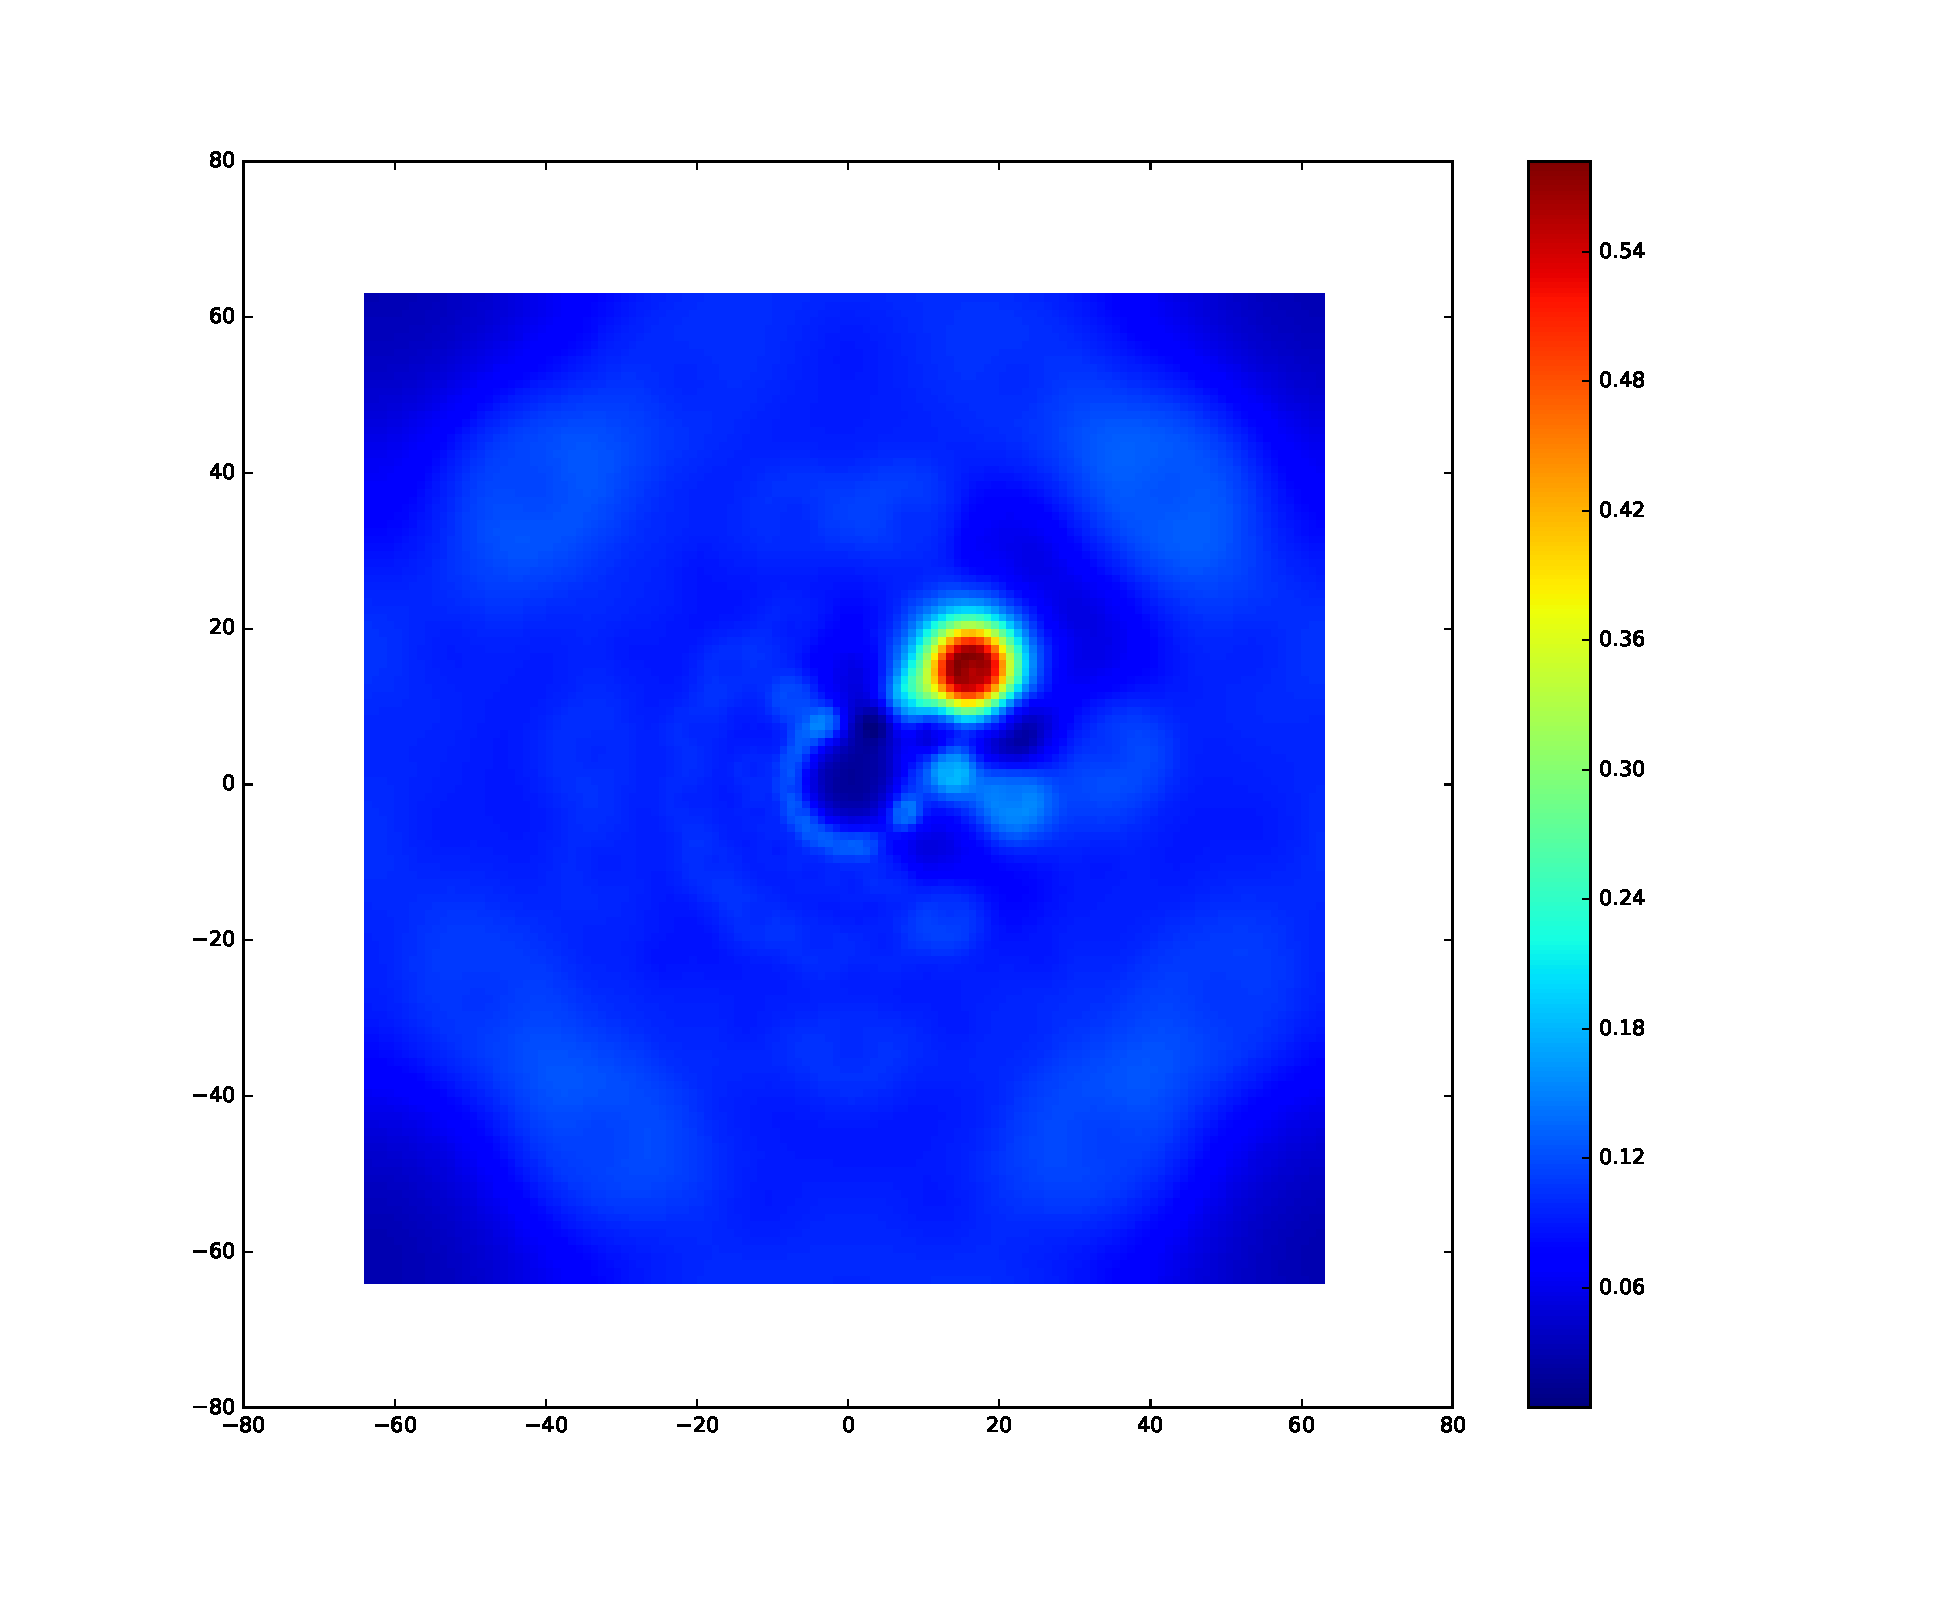
\includegraphics[scale=0.4]{Figures/accuracy_128_LP}
\decoRule
\caption[Figure]{Reconstruction en carte de chaleur de la carte de certitude après passage dans le filtre rétinien LogPolaire}
\label{fig:accuracy_128_LP}
\end{figure}

%%%%% Résultats %%%%%
